\PassOptionsToPackage{unicode=true}{hyperref} % options for packages loaded elsewhere
\PassOptionsToPackage{hyphens}{url}
%
\documentclass[]{article}
\usepackage{lmodern}
\usepackage{amssymb,amsmath}
\usepackage{ifxetex,ifluatex}
\usepackage{fixltx2e} % provides \textsubscript
\ifnum 0\ifxetex 1\fi\ifluatex 1\fi=0 % if pdftex
  \usepackage[T1]{fontenc}
  \usepackage[utf8]{inputenc}
  \usepackage{textcomp} % provides euro and other symbols
\else % if luatex or xelatex
  \usepackage{unicode-math}
  \defaultfontfeatures{Ligatures=TeX,Scale=MatchLowercase}
\fi
% use upquote if available, for straight quotes in verbatim environments
\IfFileExists{upquote.sty}{\usepackage{upquote}}{}
% use microtype if available
\IfFileExists{microtype.sty}{%
\usepackage[]{microtype}
\UseMicrotypeSet[protrusion]{basicmath} % disable protrusion for tt fonts
}{}
\IfFileExists{parskip.sty}{%
\usepackage{parskip}
}{% else
\setlength{\parindent}{0pt}
\setlength{\parskip}{6pt plus 2pt minus 1pt}
}
\usepackage{hyperref}
\hypersetup{
            pdftitle={Project 2: Breast Cancer Prediction Model},
            pdfauthor={Group 7: Melanie Mayer, Yuqi Miao, Sibei Liu, Xue Jin},
            pdfborder={0 0 0},
            breaklinks=true}
\urlstyle{same}  % don't use monospace font for urls
\usepackage[margin=1in]{geometry}
\usepackage{graphicx,grffile}
\makeatletter
\def\maxwidth{\ifdim\Gin@nat@width>\linewidth\linewidth\else\Gin@nat@width\fi}
\def\maxheight{\ifdim\Gin@nat@height>\textheight\textheight\else\Gin@nat@height\fi}
\makeatother
% Scale images if necessary, so that they will not overflow the page
% margins by default, and it is still possible to overwrite the defaults
% using explicit options in \includegraphics[width, height, ...]{}
\setkeys{Gin}{width=\maxwidth,height=\maxheight,keepaspectratio}
\setlength{\emergencystretch}{3em}  % prevent overfull lines
\providecommand{\tightlist}{%
  \setlength{\itemsep}{0pt}\setlength{\parskip}{0pt}}
\setcounter{secnumdepth}{0}
% Redefines (sub)paragraphs to behave more like sections
\ifx\paragraph\undefined\else
\let\oldparagraph\paragraph
\renewcommand{\paragraph}[1]{\oldparagraph{#1}\mbox{}}
\fi
\ifx\subparagraph\undefined\else
\let\oldsubparagraph\subparagraph
\renewcommand{\subparagraph}[1]{\oldsubparagraph{#1}\mbox{}}
\fi

% set default figure placement to htbp
\makeatletter
\def\fps@figure{htbp}
\makeatother


\title{Project 2: Breast Cancer Prediction Model}
\author{Group 7: Melanie Mayer, Yuqi Miao, Sibei Liu, Xue Jin}
\date{March 31, 2020}

\begin{document}
\maketitle

\hypertarget{introduction}{%
\subsubsection{Introduction}\label{introduction}}

Breast cancer is the most common invasive cancer and the second leading
cause of death from cancer in women worldwide, marked by the
uncontrolled growth of breast cells. Non-cancerous breast tumors do not
metastasize and are usually not life-threatening, while malignant tumors
are cancerous, aggressive and deadly. Therefore, it's important to have
breast lumps accurately diagnosed so that decision with regard to
medical treatment, rehabilitation and personal matters can be made
appropriately.

\hypertarget{objectives}{%
\subsubsection{Objectives}\label{objectives}}

The main objective of this project is to build an accurate predictive
model based on logistic regression that classifies between malignant and
benign images of breast tissue. Using the Breast Cancer Diagnosis
dataset, logistics model and logistic-LASSO model will be implemented to
predict the diagnosis. A Newton-Raphson algorithm and Pathwise
Coordinate optimization will be developed to estimate the logistic model
and the lasso model respectively. We aim to find the model with the best
performance in terms of predicting when breast tissue is malignant.

\hypertarget{breast-cancer-diagnosis-dataset}{%
\subsubsection{Breast Cancer Diagnosis
Dataset}\label{breast-cancer-diagnosis-dataset}}

The Breast Cancer Diagnosis dataset, with 569 observations, contains the
diagnosis and a set of 10 features capturing the characteristics of the
cell nuclei present in the digitized image of breast mass. The ten
features collected for each cell nucleus are:

\begin{itemize}
\tightlist
\item
  radius (mean of distances from center to points on the perimeter)
\item
  texture (standard deviation of gray-scale values)
\item
  perimeter
\item
  area
\item
  smoothness (local variation in radius lengths)
\item
  compactness (perimeter\^{}2 / area - 1.0)
\item
  concavity (severity of concave portions of the contour)
\item
  concave points (number of concave portions of the contour)
\item
  symmetry
\item
  fractal dimension (``coastline approximation'' - 1)
\end{itemize}

The mean, standard deviation (SD) and largest values of these features
are computed for each image, resulting in 30 possible predictive
variables. We will analyze the predictive ability for diagnosis of
malignant or benign cases of these covariates. The mean of each feature
will be included in our models and presented in the result section. We
will also create models with all 30 predictors however, these results
will be reported in the supplement section.

\hypertarget{methods}{%
\subsubsection{Methods}\label{methods}}

\hypertarget{model-parameters}{%
\paragraph{Model Parameters}\label{model-parameters}}

For logistic regression we assume the response variable \(Y_i\) for the
\(i_{th}\) observation follows a binary distribution:

\[Y_i\sim Bin(\pi_i)\] where \(\pi_i\) denotes the probablity that the
\(i_{th}\) observation's tissue is malignant. We can assume all
observations are independent from one another, hence the likelihood
function for the vector \(\boldsymbol\pi\) can be written as:

\[L(\boldsymbol\pi)=\prod_{i=1}^n f(y_i)=\prod_{i=1}^n\pi_i^{y_i}(1 - \pi_i)^{1-y_i}\]

For logistic regression, the logit link function is used:

\[\log(\frac{\pi_i}{1-\pi_i}) = \boldsymbol \beta ^T\boldsymbol x_i = \theta_i\]
where
\(\boldsymbol x_i^T = \begin{bmatrix} 1 & x_{1i} &x_{2i} & ... & x_{pi} \end{bmatrix}\)
and
\(\boldsymbol \beta^T = \begin{bmatrix} \beta_0 & \beta_1 & \beta_2 & ... & \beta_p \end{bmatrix}\).
One can solve for \(\pi_i = \frac{e^{\theta_i}}{1 + e^{\theta_i}}\). We
aim to find the best estimate of the vector of coefficients,
\(\boldsymbol \beta\). The log-likelihood function for this vector can
be written as:

\[l(\boldsymbol\theta)=logL(\boldsymbol\pi) =\sum_{i=1}^n(Y_ilog\frac{\pi_i}{1-\pi_i}+log(1-\pi_i)) = \sum_{i=1}^n(Y_i\theta_i - log(1 + e^{\mathbf \theta_i}))\\\]
The maximum likelihood is thus achieved when the gradient is equal to
zero and the Hessian is negative definite. The gradient can be found to
be:

\[\nabla l(\boldsymbol\theta|\boldsymbol X) = \sum_{i=1}^n (Y_i - \pi_i)\boldsymbol x_i = \boldsymbol X^T(\boldsymbol Y - \boldsymbol \pi) \]

The Hessian matrix is thus:

\[\nabla^2 l(\boldsymbol\theta|\boldsymbol X) = -\sum_{i=1}^n \pi_i(1 - \pi_i)\boldsymbol x_i\boldsymbol x_i^T = -\boldsymbol X^Tdiag(\pi_i(1 - \pi_i)) \boldsymbol X\]

\hypertarget{full-model}{%
\paragraph{Full model}\label{full-model}}

In order to estimate \(\boldsymbol \beta\) we need to maximize the
loglikelihood function. There is no closed form, hence we turn to
numerical methods. The Newton-Raphson method is used to fit the full
logistic model. To find the maximum likelihood estimate of each element
of \(\boldsymbol \beta\), an iterative process is set as follows:

\[\theta_{i+1}  = \theta_{i} -\delta (\nabla^2l(\theta_{i}|\boldsymbol X)-\gamma I)^{-1}\nabla l(\theta_{i}|\boldsymbol X) \]
This is the Newton-Raphson method with two modifications. \(\delta\) is
included in the process to accomplish the step-halving modification, the
step coefficient ensures the likelihood is always increasing in order to
achieve quicker convergence. Once the likelihood approaches convergence
the steps become smaller until convergence is reached. \(\gamma\) is the
modification coefficient to ensure the aescent direction of the
iteration vector at \(\theta_{i}\).

\hypertarget{logit-lasso-pathwise-coordinate-wise-update-algorithm}{%
\paragraph{Logit-lasso Pathwise Coordinate-wise Update
Algorithm}\label{logit-lasso-pathwise-coordinate-wise-update-algorithm}}

In the case of large dimensionality or multicollinearity of predictors
it can be beneficial to perform a regularization method which shrinks
coefficients and can perform variable selection. Here we implement the
Least Absolute Shrinkage and Selection Operator (LASSO) method for
logistic regression with a path-wise coordinate-wise optimization
algorithm to select variables from the full model, increase the
prediction efficiency and avoid overfitting. With the ten predictor
model, LASSO may not be as beneficial compared to the 30 predictor model
where we have 30 predictors describing 10 features hence are likely to
experience multicollinearity and expect LASSO to outperform the
classical logistic regression.

In LASSO we add an L1 penalization term to the loss function, such that
we try to find the coefficients to minimize:

\[min _{(\boldsymbol \beta)}\{-l({\boldsymbol \beta})+\lambda\sum_{j=0}^{p}|\beta_j| \}\]
With the pathwise coordinate-wise update algorithm, we find the
likelihood to be:
\[l({\boldsymbol \beta}) = -\frac{1}{2n}\sum_{i=1}^{n}\omega_i(z_i-{\boldsymbol {X_i\beta}})^2\]
where,
\[\pi_i = \frac{exp({\boldsymbol {X_i\beta}})}{1+exp({\boldsymbol {X_i\beta}})}\]

\[\omega_i = \pi_i(1-\pi_i)\]

\[z_i = {\boldsymbol {X_i\beta}}+\frac{y_i-\pi_i}{\pi_i(1-\pi_i)}\]

One must pre-define the tuning parameter sequence
\(\{\lambda_1,...,\lambda_s\}\) and a starting vector
\({\boldsymbol{\beta_{start=}}}\{\beta_0^{(0)},...,\beta_p^{(0)}\}\).
When choosing the sequence of lambdas, it is best to define
\(max{(\boldsymbol \lambda)} = max(\boldsymbol\beta)\), where
\(\boldsymbol\beta\) refers to the estimated coefficients from the
logistic regression, such that all coefficients will shrink to zero. The
optimal process for each \(\lambda_u\) is then found by using the
optimal \(\boldsymbol {\beta_{u-1}}\) from the previous iteration as a
warm start in order to reach the optimal values quicker. Within every
iteration for each lambda, the optimal \(\boldsymbol \beta\) is searched
using coordinate-wise updating, that is it is minimized over one
parameter at a time while keeping all others fixed.

For \(\beta_j\) in \(t_{th}\) iteration

\[\beta_j^{(t)} = \left\{\begin{array}{lc} \frac{\sum_{i=1}^{n} \omega_i(z_i-\sum_{j=1}^{p}{\boldsymbol {X_i}\beta_j})}{\sum_{i}^{n}\omega_i},&j=0\\\frac{s(\beta_j^{(t*)},\lambda_un)}{\sum_{i=1}^{n}\omega_ix_{ij}^2},&j = 1,2,...,p\end{array}\right.\]

\[\beta_j^{(t*)} = \sum_{i=1}^{n}\omega_ix_{ij}z_{ij}^*\]
\[z_{ij}^* = z_i-\underset {\beta_k\neq0}{\sum_{k = 0}^{j-1}}\beta_k^{(i)}x_{ik}-\underset {\beta_k\neq0}{\sum_{k=j+1}^{p}}\beta_k^{(i-1)}x_{ik}\]

\hypertarget{cross-validation}{%
\paragraph{Cross Validation}\label{cross-validation}}

In order to find the optimal lambda, we use 5-fold cross validation. The
dataset is divided into five subdatasets. The optimal coefficients is
then found five times by running the logit-LASSO on a combination of
four of the five subsets, leaving a different subset out each time. The
subset left out is then used to estimate the model performance. This is
done for all lambdas in the pre-defined sequence in order to search for
the lambda with the highest average predictive ability. The statistics
we use to compare predictive ability is SSE and pearson chi-square
statistic. SSE is defined as:

\[SSE = \sum_{i=1}^{n}(y_i-{\widehat \pi_i})^2\] where
\({\widehat \pi_i} = log\frac{exp({\boldsymbol X_i\beta})}{1+exp({\boldsymbol X_i\beta})}\).
Pearson chi-square statistic is defined as:
\[G = \sum_{i=1}^{n}\frac{y_i-{\widehat \pi_i}}{{\widehat \pi_i}(1-{\widehat \pi_i})}\]

We want both of these statistics to be minimized. By taking the average
of the above statistics over the value found for each of the five folds,
we get a value to evaluate the model fit for each lambda.

\hypertarget{results}{%
\subsubsection{Results}\label{results}}

\hypertarget{logistic-regression-model}{%
\paragraph{Logistic Regression Model}\label{logistic-regression-model}}

The results from the logistic model estimated using the modified
Newton-Raphson algorithm with step-halving and gradient ascent can be
found in Table 1. Here we are showing the results when only using the
means of the ten features as predictors. We found average area had the
largest coefficient. For a one unit increase in the average area of the
tissue, we expect to see a change in the log odds of having a malignant
tutor of 14, holding all other predictors constant. The predictors were
all standardized so caution must be used when analyzing these
coefficients however, this seems to be very high however. The smallest
coefficient, -7.22, was estimated for average radius. The results from
logistic regression using the mean, SD and largest values of the 10
features (30 predictors) are shown in Supplementary Table 1.

\begin{center}
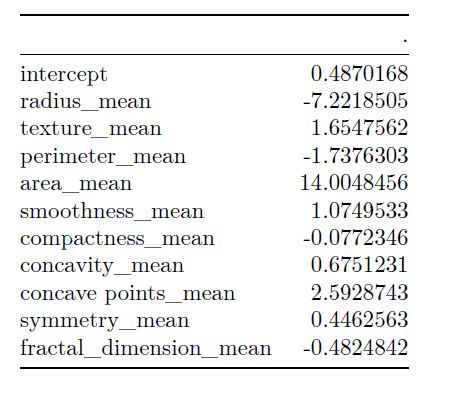
\includegraphics{./results/NR.JPG}
\end{center}

\begin{center}
Table 1. Estimated coefficients of 10 mean features under Newton-Raphson method
\end{center}

\hypertarget{logistic-lasso-model}{%
\paragraph{Logistic-LASSO Model}\label{logistic-lasso-model}}

The sequence of \(\lambda\) we compared ranged from three to zero, with
a length of 100. The pre-defined values for all \(\beta\) coefficients
including the intercept was 0.02. The optimal \(\lambda\) was selected
based on the minimum SSE, maxmimum AUC and minimum g-statistics
estimated on the test dataset. The results from each of the five folds
can be found in Table 2.

\begin{center}
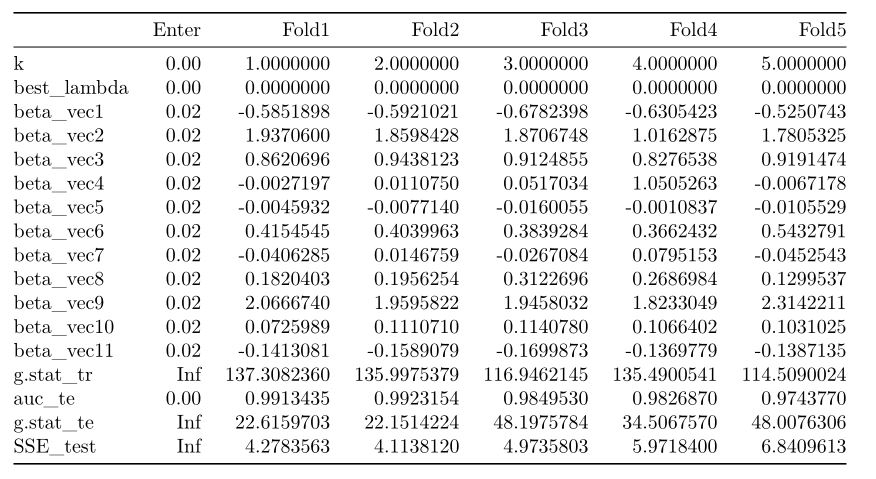
\includegraphics{./results/Results from Yuqi.JPG}
\end{center}

\begin{center}
Table 2. Cross validatin results in each fold
\end{center}

We find the results are consistant across all five folds based on all
three statistics. The optimal \(\lambda\) appears to be zero. This
implies the L1 penalization term added to the loss function is not
effecting our model. Using the test data of each fold, the AUC ranges
from 0.99 to 0.97, the g-statistic ranges from 22.6 to 48.0, while SSE
ranges from 4.1 to 6.8.

\begin{center}
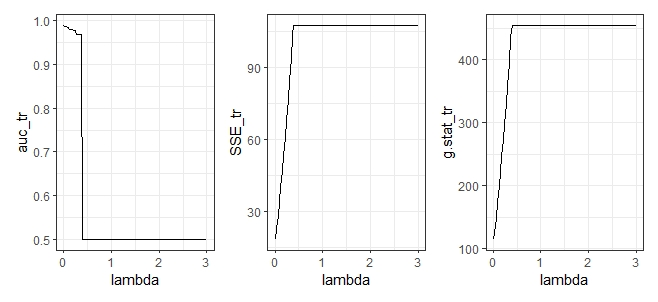
\includegraphics{./results/lambda_change.jpeg}
\end{center}

\begin{center}
Fig 1. Changes in three criteria over range of $\lambda$
\end{center}

Figure 1 shows the trend in AUC, SSE and g-statistic over the range of
lambdas tested. With the increase of \(\lambda\), both SSE and
g-statistics have a dramatic increase and become constant around 0.4.
AUC decreases drastically from 1 to 0.4. All of them indicate that the
bigger the \(\lambda\) is, the worse the model performs.

Since the optimal \(\lambda\) = 0, none of the coefficients of the
logistic-lasso is shrunk to zero, as seen in Table 3. The coefficient
terms are much smaller compared to those estimated by the classic
logistic regression however.

\begin{center}
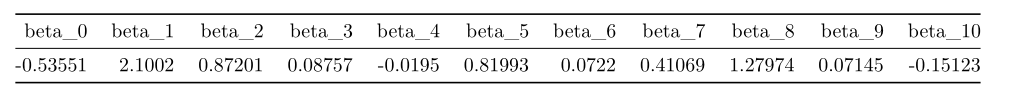
\includegraphics{./results/10 coed when lambd=0.png}
\end{center}

\begin{center}
Table 3. Coefficients of final logistic-LASSO model using cross validation
\end{center}

The results when all 30 predictors are considered, and their
corresponding Cross Validation results in each fold, are shown in
Supplementary Table 2. The optimal \(\lambda\) under that scenario is
0.03, which shrinks about 20 coefficients to 0, as presented in
Supplementary Table 3.

\hypertarget{discussion}{%
\subsubsection{Discussion}\label{discussion}}

When attempting to estimate a binary outcome, there are many other
models which could have been used. We could have compared our results to
other generalized linear models using a probit or complementary log-log
link function.

\hypertarget{supplement}{%
\subsubsection{Supplement}\label{supplement}}

\begin{center}
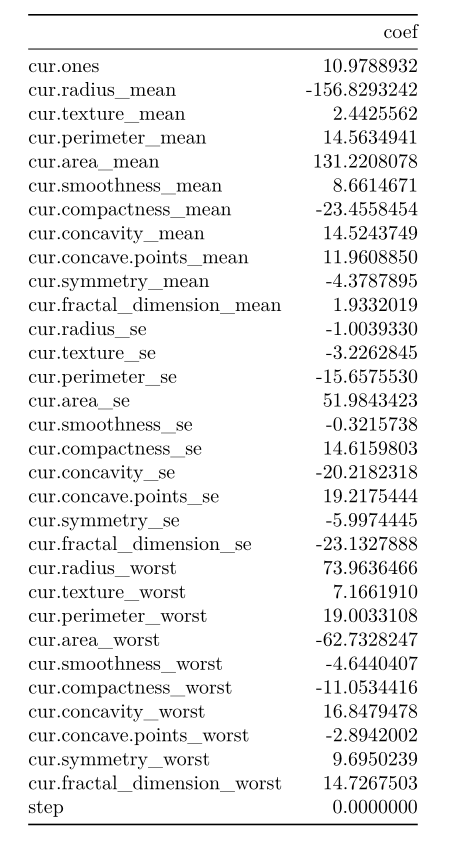
\includegraphics{./results/coef in NR of all 30 predictors.png}
\end{center}

\begin{center}
Supplementary Table  1: Estimated coefficients of 30 features under Newton-Raphson method
\end{center}

\begin{center}
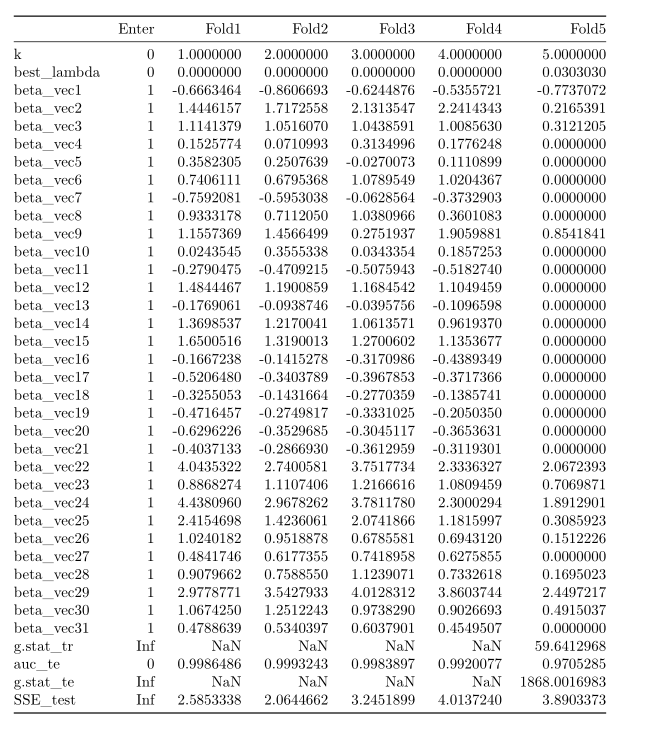
\includegraphics{./results/coef of all 30 predictors in logistic lasso.png}
\end{center}

\begin{center}
Supplementary Table 2: Estimated coefficients of 30 features in each fold of Cross Validation
\end{center}

\begin{center}
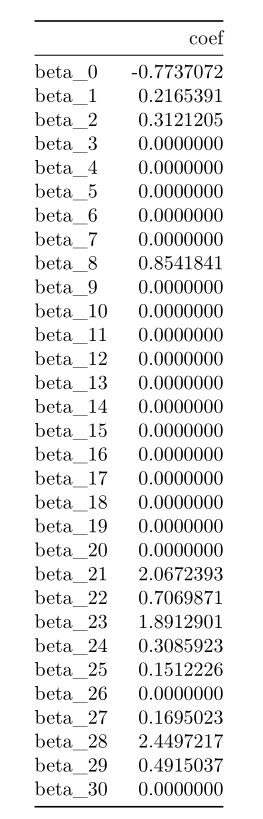
\includegraphics{./results/30 coefs when lambda=0.03.png}
\end{center}

\begin{center}
Supplementary Table 3: Estimated coefficients of 30 features in final model in Cross Validation
\end{center}

\end{document}
